\chapter{Introduction}

This document describes how to compile an \ee\ application from the
Microchip MPLAB IDE, which is the de facto standard for compilation
and debugging \dspic\ source code.

The procedure described in this document does not use the \rtd\
Eclipse graphical interface, and proposes a development flow which
nicely integrates with MPLAB IDE.

The development process we propose can be described as follows:
\begin{itemize}

\item The user has to write an OIL File to properly configure the \ee\
	kernel;

\item The user generates a custom library from an OIL File. Generating
	a custom library for each OIL file ensures that the
	application will only link useful code to the final binary
	image, making this way a good usage of the scarce resources
	which are available on the microcontrollers;

\item Finally, the user either uses an MPLAB IDE project file
	generated by the scripts, or creates an MPLAB IDE project as
	usual, including the library and the include files path in the
	final application.
\end{itemize}

\chapter{Installing \ee\ and \rtd\ on Microsoft Windows}
\label{cha:installing}

This document subsumes that the \ee\ has been correctly installed in
your system.

If you did not install \ee\ yet, please follow the install instruction
which you can find in the document "\ee\ Tutorial for the \dspic\
platform" which is installed together with \ee\ and which can also be
found in the Evidence website.

\chapter{Building the \ee\ library}

The main idea of this step is that from an OIL configuration file it
is possible to generate a customized library which contains a copy of
the \ee\ code which will be used in the final application. This
ensures that the final application will only contains the needed code,
optimizing in this way the final system footprint.

To create an \ee\ library from an OIL File, you need to follow these steps:
\begin{enumerate}
\item 
  Open a Windows command shell;

\item 
  "cd" in the Evidence bin directory with the following command (We
  suppose that \ee\ has been installed in \file{c:\\Program
  Files\\Evidence}:

\begin{lstlisting}
cd c:\Program Files\Evidence\bin
\end{lstlisting}

\item
  Execute a batch file to generate the library from an OIL file, with the following command:

\begin{lstlisting}
mplab_generatelib.bat oilfile.oil destdir
\end{lstlisting}

where \file{oilfile.oil} is the OIL File to be used, and
\file{destdir} is an empty directory that will store the results of
the compilation.

\begin{warning} 

Both \file{oilfile.oil} and \file{destdir} are absolute
pathnames. \file{destdir} will be created if not existent. If the
names contain spaces, please surround them by double quotes, like in
the following example (Note: put the three lines on a single line!):

\begin{lstlisting}
mplab_generatelib.bat 
  "C:\mydir with spaces\file.oil"
  "C:\mydir with spaces\mydirectory"
\end{lstlisting}

\end{warning}

\item
  As a result, a batch script is run (see Figure
  \ref{fig:mplab-support1}), and two directories are created
  inside \file{destdir}. The first directory, \file{Debug}, contains
  the products of the compilation process, and it has the same
  contents as what is typically generated in \rtd\ when building a
  project. After the execution of the batch script, it is not
  necessary to retain the \file{Debug} directory (unless you want to
  get access to debug information for the \ee\ source code).

  The second directory, \file{Files}, contains the files which are
  imported and used from MPLAB IDE. In particular, it contains the
  application include files, and the compiled library.

  Moreover, the destination directory contains a Microchip MPLAB IDE
  project file, which will be used in the next steps.

%
\begin{figure}[htb]
\begin{center}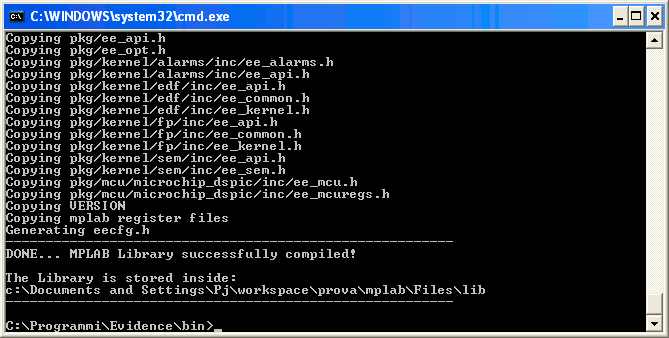
\includegraphics[
  width=12cm, bb=0 0 669 338]{images/mplab_support1.png}\end{center}
\caption{The result of the execution of the \file{mplab_generatelib.bat} batch file.}
\label{fig:mplab-support1}
\end{figure}

\item
  At this point, open MPLAB IDE and open the MPLAB IDE project file
  which has been generated by the script in the destination
  directory. 

  As an alternative, you can generate your own MPLAN IDE
  Project by following these steps:

  \begin{enumerate}
  \item 
    Open MPLAB IDE.

  \item
    Create a new Project.

  \item
    Add the \file{libee.a} library which has been generated by the
    batch script under \file{destdir\\Files\\lib\\libee.a} to the
    project. To do that, select "Add Files to Projects..." in the
    "Project" menu (see Figure \ref{fig:mplab-support2}). Then, select
    the \file{destdir\\Files\\lib\\libee.a} (see Figure
    \ref{fig:mplab-support3}).

%
\begin{figure}[htb]
\begin{center}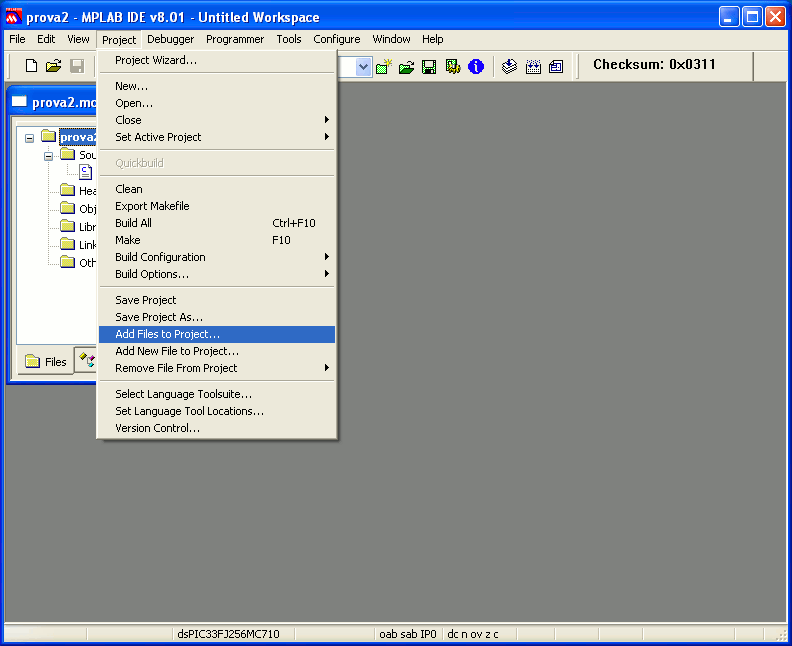
\includegraphics[
  width=12cm, bb=0 0 792 646]{images/mplab_support2.png}\end{center}
\caption{Add Files to the Project...}
\label{fig:mplab-support2}
\end{figure}
%
\begin{figure}[htb]
\begin{center}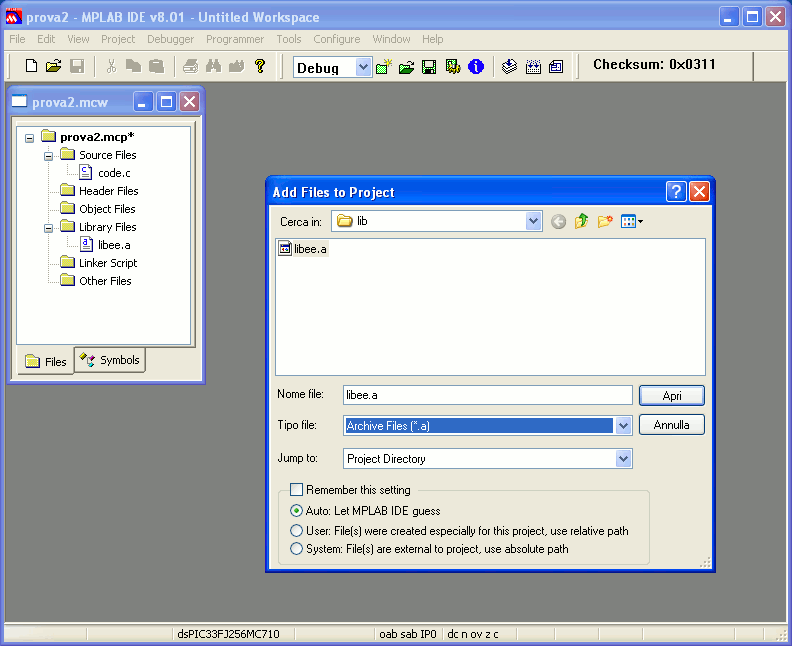
\includegraphics[
  width=12cm, bb=0 0 792 646]{images/mplab_support3.png}\end{center}
\caption{Add the Library file to the project.}
\label{fig:mplab-support3}
\end{figure}

  \item
    After that, you need to modify the Project Build Options by adding
    an include directory and setting the ELF format. To do that,
    select "Build Options..."/"Project" under the "Project" menu (see
    Figure \ref{fig:mplab-support4}). Then, add the
    \file{destdir\\Files\\pkg} as an include directory path (see Figure
    \ref{fig:mplab-support5}), and select ELF as output file format
    (see Figure \ref{fig:mplab-support6}).

%
\begin{figure}[htb]
\begin{center}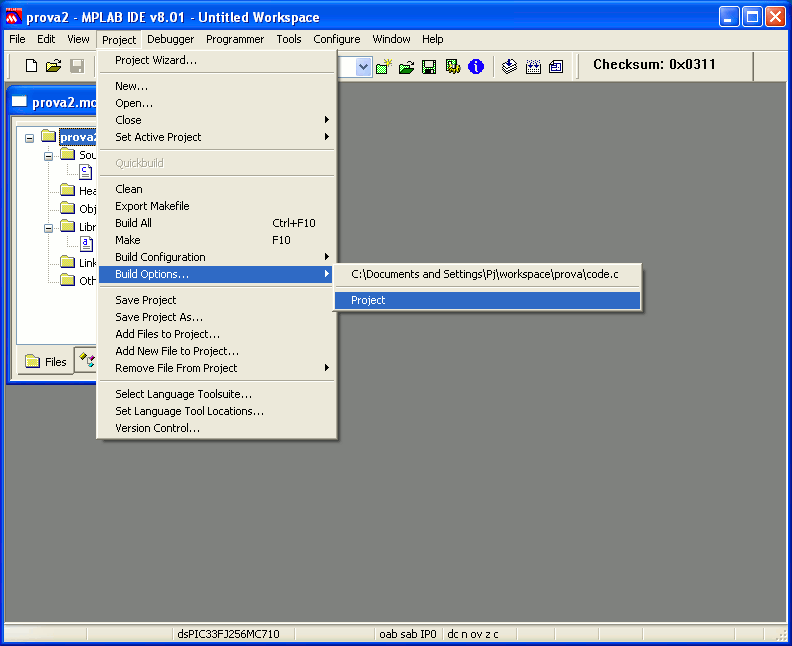
\includegraphics[
  width=12cm, bb=0 0 792 646]{images/mplab_support4.png}\end{center}
\caption{Set the project build options.}
\label{fig:mplab-support4}
\end{figure}
%
\begin{figure}[htb]
\begin{center}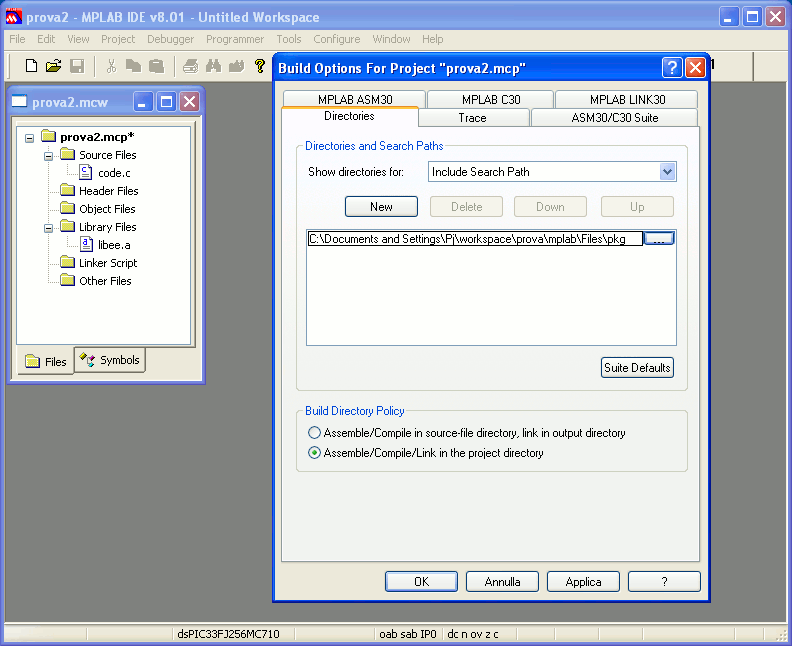
\includegraphics[
  width=12cm, bb=0 0 792 646]{images/mplab_support5.png}\end{center}
\caption{Set the additional Include path.}
\label{fig:mplab-support5}
\end{figure}
%
\begin{figure}[htb]
\begin{center}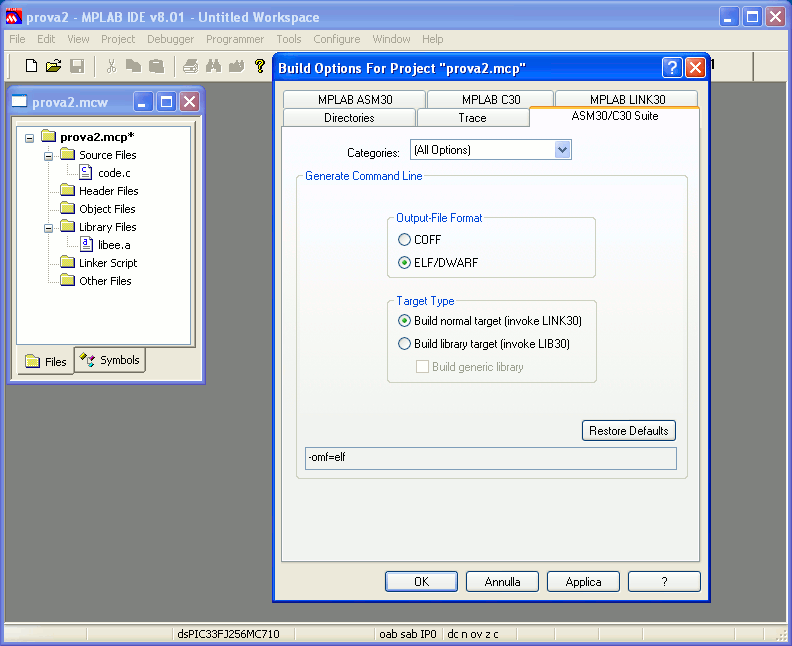
\includegraphics[
  width=12cm, bb=0 0 792 646]{images/mplab_support6.png}\end{center}
\caption{Set the output file format.}
\label{fig:mplab-support6}
\end{figure}

  \end{enumerate}




\item
  Add your application files, and compile it as usually done with MPLAB IDE. The result will be similar to what showed in Figure \ref{fig:mplab-support7}.

%
\begin{figure}[htb]
\begin{center}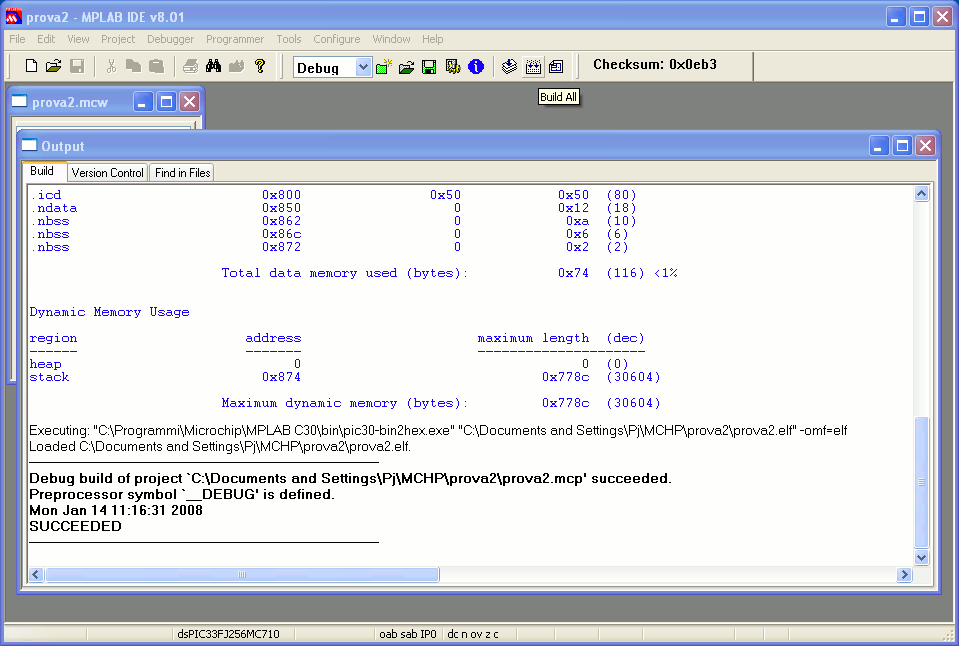
\includegraphics[
  width=12cm, bb=0 0 959 646]{images/mplab_support7.png}\end{center}
\caption{The result of the application compilation on MPLAB IDE.}
\label{fig:mplab-support7}
\end{figure}

\end{enumerate}

